\documentclass[
  a4paper,
  12pt,
  spanish,
]{scrartcl}

% Párrafos
\setlength{\parindent}{18pt}
\linespread{1.05}

%-------------------------------------------------------------------------------
%	PAQUETES
%-------------------------------------------------------------------------------

% Idioma

\usepackage[es-noindentfirst, es-tabla]{babel}

% Citas de texto en línea/bloque

\usepackage[autostyle]{csquotes}

% Tablas

\usepackage{booktabs}
\usepackage{multirow}

% Matemáticas

\usepackage{amsmath, amsthm, amssymb}
\usepackage{mathtools}
\usepackage{commath}

% Fuentes personalizadas para utilizar con XeLaTeX o LuaLaTeX

\usepackage[no-math]{fontspec}
\setmainfont{Libertinus Serif}
\setsansfont{Libertinus Sans}
\setmonofont{Libertinus Mono}

\usepackage[math-style=TeX]{unicode-math}
\setmathfont{Libertinus Math}

% Configuración de microtype

\defaultfontfeatures{Ligatures=TeX,Numbers=Lining}
\usepackage[activate={true,nocompatibility},final,tracking=true,factor=1100,stretch=10,shrink=10]{microtype}
\SetTracking{encoding={*}, shape=sc}{0}

% Enlaces y colores

\usepackage{hyperref}
\usepackage[dvipsnames]{xcolor}
\definecolor{webgreen}{rgb}{0,0.5,0}
\hypersetup{
  colorlinks=true,
  citecolor=webgreen,
  urlcolor=Maroon,
  linkcolor=RoyalBlue
}

% Otros elementos de página

\usepackage{enumitem}
\setlist[enumerate]{leftmargin=*, itemsep=0pt}
\setlist[itemize]{leftmargin=*, itemsep=0pt}

\usepackage[labelfont=sc]{caption}

% Tikz

\usepackage{tikz}
\usetikzlibrary{babel}
\usepackage{float}

% Código

\usepackage{listings}
\lstset{
	basicstyle=\footnotesize\ttfamily,%
	breaklines=true,%
	captionpos=b,                    % sets the caption-position to bottom
  tabsize=2,	                   % sets default tabsize to 2 spaces
  frame=lines,
  numbers=left,
  stepnumber=1,
  aboveskip=12pt,
  showstringspaces=false,
}
\renewcommand{\lstlistingname}{Listado}

% Algoritmos

\usepackage[linesnumbered, vlined]{algorithm2e}
\SetAlFnt{\sffamily}
\newcommand{\mykwfont}{\bfseries\sffamily}
\SetKwSty{mykwfont}

\SetKwInput{KwIn}{Entrada}%
\SetKwInput{KwOut}{Salida}%

\SetAlCapSkip{1em}
\SetAlCapFnt{\normalfont\scshape}

% Bibliografía

\usepackage[sorting=none, style=apa, isbn=true]{biblatex}
\DefineBibliographyStrings{spanish}{
  urlseen = {Consultado},
  retrieved = {Consultado},
}
\addbibresource{bibliografia.bib}

% Lorem ipsum

\usepackage{blindtext}

% Márgenes
\usepackage[bottom=3.125cm, top=2.5cm, left=4.5cm, right=4.5cm, marginparwidth=70pt]{geometry}

% Fuentes

\usepackage{textcase}

\newfontfamily{\sacshape}{Libertinus Serif}[
  WordSpace={1.8},
  LetterSpace={18.0}
]

\newfontfamily{\slscshape}{Libertinus Serif}[
  WordSpace={1.8},
  LetterSpace={6.0}
]

\DeclareRobustCommand{\spacedallcaps}[1]{{\linespread{1.3}\sacshape\MakeTextUppercase{#1}}}% WordSpace=1.8
\DeclareRobustCommand{\spacedlowsmallcaps}[1]{{\slscshape\MakeTextLowercase{#1}}}% WordSpace=1.8

% Cabeceras de sección

\RedeclareSectionCommands[beforeskip=-3ex,
afterskip=2ex]{section,subsection,subsubsection}
%\addtokomafont{section}{\normalfont\large\spacedallcaps}
%\setkomafont{section}{\normalfont\large\scshape}
\RedeclareSectionCommand[beforeskip=-9ex, font=\normalfont\large\scshape, tocentryformat=\normalfont\scshape]{section}
\addtokomafont{subsection}{\normalfont\normalsize\itshape}
\RedeclareSectionCommand[beforeskip=-6ex,tocentryformat=\normalfont\itshape]{subsection}
\addtokomafont{subsubsection}{\normalfont}
\RedeclareSectionCommand[beforeskip=-4ex]{subsubsection}
\addtokomafont{paragraph}{\normalfont\itshape}

%-------------------------------------------------------------------------------
%	TÍTULO
%-------------------------------------------------------------------------------

\newcommand{\horrule}[1]{\rule{\linewidth}{#1}}

%-------------------------------------------------------------------------------
%	CONTENIDO
%-------------------------------------------------------------------------------

\begin{document}

\begin{titlepage}
  \vspace*{4cm}

  \begin{flushleft}
    \Huge
    \spacedallcaps{Curvas Elípticas en la Criptografía}
    \horrule{2pt}
  \end{flushleft}

  \vspace{2em}

  \begin{flushright}
    \large
    Sofía Almeida Bruno\\
    Antonio Coín Castro\\
    José María Martín Luque\vspace{1em}

    \textit{Historia de las Matemáticas}

    Grado en Matemáticas

    \textsc{Universidad de Granada}\vspace{1em}

    \today\vspace{.5em}
  \end{flushright}
\end{titlepage}

\newpage

{\hypersetup{hidelinks}
\tableofcontents
}

\newpage

\section{Introducción}

El objetivo principal de la criptografía es la transmisión de información confidencial a través de un canal inseguro. Ya desde la antigüedad una de las preocupaciones era el intercambio de mensajes de forma privada, sobre todo en el contexto de asuntos bélicos y políticos. Un ejemplo famoso es el \textit{cifrado de César}, que consistía en sustituir cada carácter del mensaje por otro prefijado. A lo largo de la historia se fueron desarrollando otros métodos más sofisticados, pero es con la aparición de los ordenadores y su uso en las comunicaciones cuando la investigación en este ámbito experimenta una evolución sin precedentes.

En la década de los 70 aparecen varios algortimos y protocolos para tratar de aumentar la seguridad en el intercambio de información, basados principalmente en ciertos problemas matemáticos considerados difíciles de resolver incluso con la capacidad de cómputo que introdujeron los ordenadores. Es por esto que se comenzó a adaptar diferentes herramientas matemáticas que en principio no tenían relación con la criptografía para intentar desarrollar algoritmos, sistemas y protocolos difíciles de comprometer. Un ejemplo de esto es la introducción en los sistemas criptográficos de \textit{curvas elípticas}, cuya evolución es precisamente el objeto de estudio de este trabajo.

En la Sección \ref{sec:curvas} daremos una definición general de curvas elípticas, comentaremos su estructura de grupo y estudiaremos un caso particular ampliamente utilizado en cripotografía: las curvas elípticas sobre cuerpos finitos. Continuaremos en la Sección \ref{sec:historia} con un repaso al estado de la criptografía anterior a la introducción de las curvas elípticas en ese campo, describiendo posteriormente su irrupción y evolución, que no estuvo exenta de polémica, hasta llegar a los tiempos actuales en los que gozan de gran aceptación. Finalmente, en la Sección \ref{sec:futuro} hablaremos sobre posibles usos de las curvas elípticas en un hipotético futuro dominado por los ordenadores cuánticos, cuya llegada se especula que rompería todos los esquemas criptográficos actuales y comprometería enormemente la seguridad de los sistemas informáticos.



%TODO: completar introducción

\section{Curvas elípticas}
\label{sec:curvas}

Antes de analizar la historia y el papel de las curvas elípticas en el contexto de la criptografía, damos una definición de ellas como objetos matemáticos abstractos.

    Sea $K$ un cuerpo y $\overline{K}$ su clausura algebraica. Una \textit{curva elíptica} sobre $\overline{K}$ es una curva proyectiva no singular $E \subset \mathbb{P}^2(\overline{K})$ definida por una ecuación afín de la forma \[ y^2 + a_1xy + a_3y = x^3 +a_2x^2 + a_4x + a_6, \] donde todos los $a_i \in \overline{K}$.
    Cuando la característica de $\overline{K}$ es distinta de $2$ y de $3$, podemos simplificar la ecuación como \[ y^2 = x^3 + Ax + B, \] con $A,B \in \overline{K}$. Una ecuación de esta forma se conoce como \textit{ecuación de Weierstrass}, y en este caso la condición de no singularidad implica que $4A^3 + 27B^2 \neq 0$. Si de hecho los coeficientes $A$ y $B$ están en $K$, decimos que la curva está definida sobre $K$, y nos referimos a ella como \[ E = E(K) = \{ (x, y) \in K \times K : y^2 = x^3 + Ax + B\} \cup \{\mathcal{O}\}, \] donde denotamos por $\mathcal{O}$ al punto en el infinito con coordenadas homogéneas $[0:1:0]$. En lo que sigue trabajaremos siempre con esta representación de las curvas.

En la Figura \ref{fig:curva} podemos ver algunas representaciones de curvas elípticas, mientras que en la Figura \ref{fig:parametros} vemos cómo afectan los parámetros $A$ y $B$ a la representación de las mismas.

\begin{figure}[h]
  \centering
  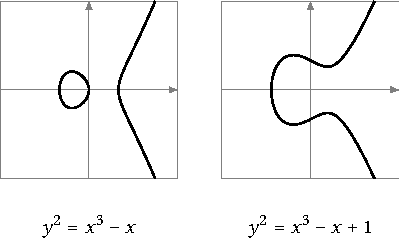
\includegraphics[width=.75\textwidth]{img/ejemplos-curvas}
  \caption{Ejemplos de curvas elípticas sobre $\mathbb{R}$. Basado en \parencite{eichlseder_elliptic_2016}.}
  \label{fig:curva}
\end{figure}

\begin{figure}[h]
  \centering
  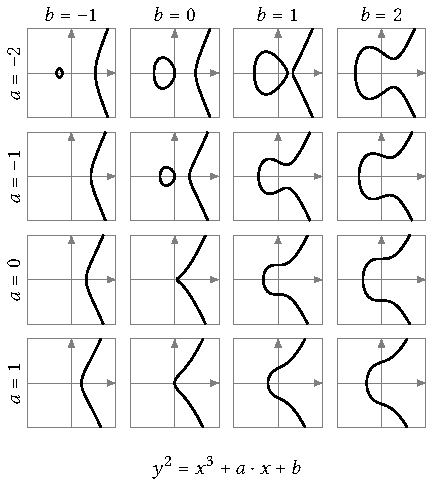
\includegraphics[width=.75\textwidth]{img/parametros-curvas}
  \caption{Ejemplos de curvas elípticas con distintos parámetros. Basado en  \parencite{eichlseder_elliptic_2016}.}
  \label{fig:parametros}
\end{figure}

\subsection{Operación de grupo en curvas elípticas}

Un detalle interesante sobre las curvas elípticas es que se puede definir sobre ellas una operación $+$ de forma que $(E, +)$ sea un grupo abeliano, con elemento identidad el punto $\mathcal{O}$. Para definir esta operación, supondremos por un momento que $K = \mathbb{R}$, y entenderemos que el punto del infinito se encuentra <<al principio>> y <<al final>> del eje de ordenadas.
Podemos pensar entonces que que una recta vertical siempre interseca a $E$ al menos en el punto \(\mathcal{O}\).

El procedimiento general es el que sigue. Dados dos puntos $P = (x_1, y_1)$ y $Q = (x_2, y_2)$ con $P,Q \in E$, consideramos la recta que los une y llamamos $R$ a la otra intersección de dicha recta con la curva $E$. Entonces, definimos $P + Q$ como el punto reflejado de $R$ con respecto al eje $X$, al que llamaremos $-R$. Notamos que este procedimiento funciona siempre que la recta considerada corte efectivamente a la curva en otro punto. Discutimos ahora los posibles casos particulares del método, que podemos visualizar en la Figura \ref{fig:operaciones-curvas}.

\begin{enumerate}
  \item En primer lugar, si $P=\mathcal{O}$ tendremos que la recta que une $P$ y $Q$ es vertical, luego interseca a la curva en el punto reflejado de $Q$, es decir, $\mathcal{O} + Q = - (-Q) = Q$. Hemos probado de camino que el punto $\mathcal{O}$ actúa como elemento identidad para la operación $+$.
  \item En lo que sigue consideraremos $P, Q \neq \mathcal{O}$. Abordamos primero el caso en el que $x_1 \neq x_2$. Entonces, la recta que une $P$ y $Q$ tiene pendiente \[ m = \frac{y_2 - y_1}{x_2 - x_1}, \] y veremos que corta a la recta en otro punto $R$ que permite aplicar el procedimiento general para calcular $P+Q$.
  \item Si $Q = P$ con segunda coordenada no nula, no podemos considerar la recta que los une, pero la aproximamos por la recta tangente a $E$ en el punto $P$. Es decir, tomando $y = y(x)$ en la expresión de la curva, podemos derivar implícitamente y obtener la pendiente de la recta tangente: \[ 2yy' = 3x^2 + A \implies m = y_1'(x_1) = \frac{3x_1^2 + A}{2y_1(x_1)}. \]  Veremos también que la recta tangente corta a la curva en otro punto y podremos aplicar el procedimiento general, computando el valor de $P + P$.
  \item Por último, consideramos el caso $Q = -P$, pues al ser las curvas simétricas respecto al eje $X$ no hay otra posibilidad. Así, la recta que une $P$ y $-P$ es vertical, corta a la curva en $\mathcal{O}$, y por tanto $P + (-P) = -\mathcal{O} = \mathcal{O}$, obteniendo que el elemento inverso de un punto $P$ es su reflejado $-P$. En el caso en que la segunda coordenada sea nula, el punto se encuentra sobre el eje de abscisas. Consideramos de nuevo la recta tangente a $E$ en $P$, y tenemos que sigue siendo vertical y corta a la curva en $\mathcal{O}$, verificándose $P + P = \mathcal{O}$.
\end{enumerate}

\begin{figure}[h]
  \centering
  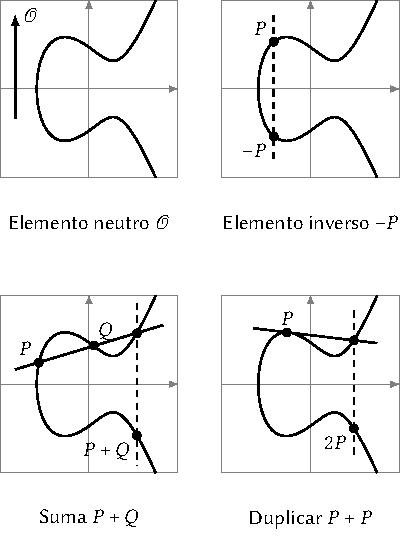
\includegraphics[width=0.65\textwidth]{img/operaciones-curvas}
  \caption{Suma de puntos en curvas elípticas. Basado en  \parencite{eichlseder_elliptic_2016}.}
  \label{fig:operaciones-curvas}
\end{figure}

Veamos ahora cómo calcular el punto de corte de la recta considerada (de pendiente $m$) con la curva $E$, en los casos que no hemos determinado explícitamente la suma de $P+Q$. Podemos escribir la recta como \[ y = m(x - x_1) + y_1, \] y para ver el punto de corte con $E$ sustituimos en su expresión, quedando: \[ (m(x - x_1) + y_1)^2 = x^3 + Ax + B. \] Simplificando esta expresión, obtenemos otra de la forma
\begin{equation}
    \label{eq:corte}
	0 = x^3 - m^2x^2 + bx + c.
\end{equation}

    Notamos que no es necesario resolver la ecuación cúbica en $x$ para determinar los puntos de corte. Si tenemos un polinomio de la forma $x^3 + ax^2 + bx + c$ y conocemos sus tres raíces $r,s,t$, podemos escribir \[ x^3 + ax^2 + bx + c = (x-r)(x-s)(x-t) = x^3 - (r+s+t)x^2 + dx + e. \] Identificando coeficientes, vemos que $-a = r + s + t$, de donde $t = -a -r -s$. Es decir, si conocemos dos raíces de la expresión, podemos conocer la tercera de forma sencilla.

    Volviendo a nuestro caso, conocemos dos soluciones de \eqref{eq:corte}, a saber, $x_1$ y $x_2$ (incluyendo el caso de solución doble $x_1=x_2$). Como $a = -m^2$, podemos calcular la tercera solución de \eqref{eq:corte} fácilmente: \[ x_3 = m^2 - x_1 - x_2. \] Por último, sustituimos en la expresión de la recta para obtener la segunda coordenada del punto de corte, es decir, \[y_3 = m(x_3 - x_1) + y_1, \] y podemos escribir $P+Q = -R$ con $R=(x_3, y_3)$.

    Para poder afirmar que $(E, +)$ es un grupo abeliano, falta verificar la conmutatividad y la asociatividad. La primera es obvia, o bien de las fórmulas desarrolladas, o bien del hecho de que la recta que une $P$ y $Q$ es la misma que la que une $Q$ y $P$. La asociatividad es algo menos trivial, pero puede comprobarse también a partir de las fórmulas para la suma. Una prueba completa puede consultarse en \parencite[sección 2.4]{elliptic_washington_2008}.

    Otra operación que podemos definir sobre puntos de curvas elípticas (y que tendrá mucha relevancia en sus aplicaciones criptográficas) es la \textit{multiplicación por escalares.} Dado un punto $P\in E$ y un natural $n$, podemos calcular \[ nP = \underbrace{P + P + \cdots + P}_{n}.\] Aunque parece que se necesitan realizar $n$ sumas, podemos calcular este punto con eficiencia $O(\log n)$ sin más que escribir $n$ en base 2 y realizar duplicaciones sucesivas. Por ejemplo, si queremos calcular $27P$, escribimos $27 = 2^4 + 2^3 + 2^1 + 2^0$, y así \[ 27P = 2^4P + 2^3P + 2P + P = 2(2^3P) + 2(2^2P) + 2P + P.\]

\subsection{Curvas elípticas sobre cuerpos finitos}

Hasta ahora hemos definido las curvas elípticas sobre un cuerpo $K$ cualquiera (o su clausura algebraica), pero es de especial interés el caso en que $K=\mathbb{F}_p$ con $p$ un primo, es decir, consideramos curvas sobre el cuerpo finito de $p$ elementos. En este caso se sigue manteniendo la estructura de grupo, teniendo en cuenta que si $Q = (x,y)$, entonces $-Q = (x, -y \bmod p)$. La operación de suma sigue teniendo las mismas expresiones algebraicas (siempre $\bmod\, p$), considerando que las rectas en $\mathbb{F}_p$ son el conjunto de puntos que verifican la ecuación \[ ax + by + c \equiv 0 \bmod p. \] Sin embargo, el método geométrico ya no es tan claro, pues no es fácil visualizar las operaciones en $\mathbb{F}_p$. Podemos ver en la Figura \ref{fig:cuerpos-curvas} una representación de una curva elíptica sobre un cuerpo finito.

\begin{figure}[h]
  \centering
  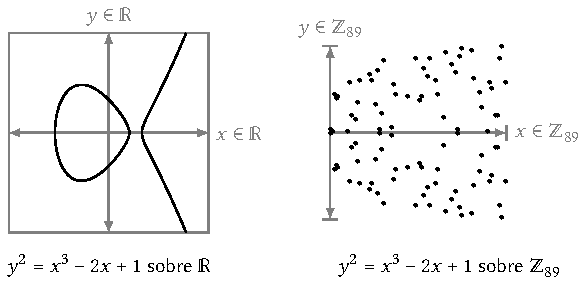
\includegraphics[width=0.85\textwidth]{img/cuerpos-curvas}
	\caption{Comparación de curvas elípticas sobre $\mathbb{R}$ y sobre $\mathbb{F}_{89}$. Basado en \parencite{eichlseder_elliptic_2016}.}
  \label{fig:cuerpos-curvas}
\end{figure}

Volviendo al problema de la multiplicación por escalares, si elegimos un punto arbitrario de la curva podemos considerar el subgrupo cíclico generado por él, que sabemos por el \textit{teorema de Lagrange} que tendrá orden un divisor del orden del grupo $(E, +)$. Existe un procedimiento llamado \textit{Algoritmo de Schoof} que permite calcular el orden de $E$ en tiempo polinómico \parencite{schoof_points_1995}.

Para nuestras aplicaciones nos interesará elegir un grupo cíclico de $E$ de orden un primo de gran tamaño, para lo cual podemos proceder de la siguiente forma:

\begin{enumerate}
	\item Calcular el orden $N$ de $E$.
	\item Escoger un factor primo $n$ de $N$.
	\item Calcular el valor $h = N/n$, que sabemos que es un número entero porque $n$ divide a $N$.
	\item Elegimos un punto cualquiera $P \in E$ y calculamos $G = hP$.
	\item Si $G=\mathcal{O}$, volvemos al punto anterior.
\end{enumerate}

Al finalizar, habremos encontrado un generador de un grupo cíclico de orden $n$, a saber, $\langle G \rangle$.

\section{Evolución de las curvas elípticas en la criptografía}
\label{sec:historia}

Un criptosistema es una familia uniparamétrica \(\{S_K\}_{K \in \{K\}}\) de aplicaciones invertibles \[S_K: \{P\} \to \{C\},\] del conjunto de mensajes en claro, \(\{P\}\), al conjunto de mensajes cifrados, \(\{C\}\).
El parámetro \(K\) se denomina \textit{clave} y el rango de posibles valores que puede tomar
%\(\{K\}\)
, \textit{espacio de claves}.

El objetivo a la hora de diseñar un criptosistema
%\(\{S_K\}\)
 ha de ser procurar que las operaciones de cifrado y descifrado resulten sencillas, asegurándose que el análisis criptográfico por parte de terceras personas con el fin de interceptar y descifrar los mensajes cifrados sea lo suficientemente difícil.

\subsection{Criptografía moderna anterior a los años 80}

En los años 70 del siglo pasado se produjeron dos acontecimientos públicos que supusieron grandes avances en el desarrollo de la criptografía moderna \parencite{singh_code_2003}, \parencite{thawte_history_2013}.

En primer lugar, en 1973 la Oficina Nacional de Normas (NBS por sus siglas en inglés, \textit{National Bureau of Standards}), dependiente del Departamento de Comercio del Gobierno Federal de los Estados Unidos, organizó un concurso público para el diseño de un algoritmo de cifrado que pudiese ser adoptado como estándar por parte de dicho Gobierno.
El 17 de marzo de 1975 se publicó el primer borrador del \textit{Data Encryption Standard} (DES), sistema de cifrado propuesto por un grupo de investigación de IBM.
Tras recibir varias modificaciones con la ayuda de la Agencia de Seguridad Nacional (NSA por sus siglas en inglés, \textit{National Security Agency}) la versión final del algoritmo fue aprobada y publicada por la NBS en noviembre de 1976 y se convirtió en el primer estándar aprobado por una agencia del Gobierno Federal de los Estados Unidos.
El hecho de que la NSA colaborase en el diseño del algoritmo --modificando la propuesta original de IBM-- suscitó las sospechas de numerosos investigadores, quienes creían que la NSA había introducido una \textit{puerta trasera} en el algoritmo.
Finalmente, en los años 90 se llegó a la conclusión de que los cambios aportados por la NSA resultaron ser mejoras.
Otra de las críticas que suscitó fue el tamaño elegido para los bloques.
En 2002 fue reemplazado por el algoritmo AES (\textit{Advanced Encryption Standard}), aprobado como estándar por el sucesor de la NBS, el Instituto Nacional de Estándares y Tecnología (NIST por sus siglas en inglés, \textit{National Institute of Standards and Technology}).

\subsubsection{Protocolo de Diffie y Hellman}

El segundo avance significativo, y el que verdaderamente es relevante para nuestro estudio, fue la publicación en 1976 del artículo \textit{New Directions in Cryptography} \parencite{diffie_new_1976} en el que los autores introducen por primera vez la idea del cifrado de clave pública.
Todo algoritmo de cifrado necesita una clave secreta, compartida únicamente entre el emisor y el receptor.
Hasta el momento la dificultad para llevar a cabo la comunicación cifrada radicaba en la transmisión de dicha clave de forma segura.
Diffie y Hellman propusieron un protocolo de intercambio de claves asimétrico que permitió resolver este problema.
Dicho protocolo utiliza una pareja de claves: una pública y otra privada, de forma que ambas partes de la comunicación pueden obtener una única clave compartida sin tener que intercambiarla de forma explícita.

La técnica se basa en la dificultad de calcular logaritmos en un cuerpo finito de \(q\) elementos, denotado \(\mathbb F_q\), siendo \(q\) un número primo.
Sea \[Y = \alpha^X \mod q, \qquad \text{para } 1 \leq X \leq q - 1,\] donde \(\alpha\) es fijo y es una \textit{raíz primitiva módulo} \(q\), es decir, todo número coprimo con \(q\) es congruente a una potencia de \(\alpha\) módulo \(q\).
Al elemento \(X\) se le llama \textit{logaritmo de} \(Y\) \textit{de base} \(\alpha\) y \textit{módulo} \(q\): \[X = \log_{\alpha} Y \mod q, \qquad \text{para } 1 \leq X \leq q - 1.\]
El cálculo de \(Y\) a partir de \(X\) es sencillo, necesitándose para ello como mucho \(2 \cdot \log_2 q\) multiplicaciones utilizando el algoritmo de \textit{exponenciación binaria}. Por ejemplo, para \(X = 18\), \[Y = \alpha^{18} = \cramped{(((\alpha^2)^2)^2)^2} \cdot \cramped{\alpha^2}.\]
Sin embargo, la operación inversa de calcular \(X\) a partir de \(Y\) es mucho más compleja, y en ello radica la seguridad de este sistema, como comentaremos más adelante.

A la hora de establecer la comunicación cifrada cada usuario genera un número aleatorio \(X_i\) de forma independiente dentro del rango de enteros \(\{1, 2, \dots, q - 1\}\).
Dicho número se conoce como \textit{clave privada} y se guarda en secreto, pero se hace público el número \[Y_i = \alpha^{X_i} \mod q,\] conocido como \textit{clave pública}.
Cuando los usuarios \(i\) y \(j\) quieren comunicarse de forma segura utilizan la clave \(K_{ij} = \cramped{\alpha^{X_iX_j}} \mod q\).
El usuario \(i\) obtiene la clave \(K_{ij}\) a partir del número público \(Y_j\) realizando las operaciones \begin{align*}
  K_{ij} &= Y_j^{X_i} \mod q \\
    &= (\alpha^{X_j})^{X_i} \mod q \\
    &= \alpha^{X_jX_i} \mod q \\
    &= \alpha^{X_iX_j} \mod q.
\end{align*}
El usuario \(j\) obtiene la clave de forma análoga, calculando en su caso \[K_{ij} = Y_i^{X_j} \mod q.\]

Observamos que el protocolo de Diffie-Hellman tiene tres parámetros: \begin{itemize}
  \item El orden del grupo, \(q\).
  \item El generador \(\alpha\) fijo.
  \item La clave \(X\) a la que elevamos \(\alpha\).
\end{itemize}

Existen varias recomendaciones sobre el tamaño de los parámetros \(q\) y \(X\). Por ejemplo la Agencia Nacional de la Seguridad de Sistemas de Información francesa (ANSSI por sus siglas en francés) hace la recomendación descrita en la Tabla \ref{tab:tam-anssi} \parencite{anssi_mecanismes_2014}, mientras que el NIST recomienda los tamaños descritos en la Tabla \ref{tab:tam-nist} \parencite{barker_recommendation_2016}.

Como se puede observar, para ofrecer niveles de seguridad significativos son necesarios tamaños de los parámetros bastante grandes. Al estudiar la criptografía de curvas elípticas veremos que los tamaños de los parámetros utilizados son mucho menores.

\begin{table}[h]
  \centering
  \sffamily
  \begin{tabular}{lcc}
    \toprule
    & \multicolumn{2}{c}{Tamaño en bits} \\
    Periodo & clave & grupo \\
    \midrule
    2014 - 2030 & 200 & 2048\\
    > 2030 & 200 & 3072\\
    \bottomrule
  \end{tabular}
  \caption{Recomendaciones de la ANSSI para el tamaño de los parámetros de Diffie-Hellman.}
  \label{tab:tam-anssi}
\end{table}

\begin{table}[h]
  \centering
  \sffamily
  \begin{tabular}{lccc}
    \toprule
     & \multicolumn{3}{c}{Tamaño en bits} \\
    Periodo & nivel de seguridad & clave & grupo \\
    \midrule
    Pasado & 80 & 160 & 1024\\
    \multirow[t]{4}{*}{2016-2030} & 112 & 224 & 2048\\
     & 128 & 256 & 3072\\
     & 192 & 384 & 7680\\
     & 256 & 512 & 15360\\
    \bottomrule
  \end{tabular}
  \caption{Recomendaciones del NIST para el tamaño de los parámetros de Diffie-Hellman. Un nivel de seguridad de \(S\) bits indica que se necesitan aproximadamente \(2^S\) operaciones para romper el cifrado.}
  \label{tab:tam-nist}
\end{table}

\subsubsection{Problema de Diffie-Hellman}

Para que una tercera persona pudiese interceptar la comunicación tendría que obtener la clave \(K_{ij}\) a partir de \(Y_i\) e \(Y_j\), para lo que tendría que calcular, por ejemplo, \[K_{ij} = Y_i^{\left(log_{\alpha} Y_j\right)} \mod q.\]
Este problema se denomina \textit{problema de Diffie-Hellman}.
En su artículo los autores conjeturan que la resolución de dicho problema es equivalente a resolver el \textit{problema del logaritmo discreto} para alguno de los valores \(Y_i\) o \(Y_j\). Este problema puede enunciarse como: \begin{displayquote}
  Sea \(G\) un grupo y \(\langle g \rangle\) el subgrupo cíclico generado por \(g\). Dado \(g \in G\) y \(a \in \langle g \rangle\), encuentra \(x\) tal que \(g^x = a\).
\end{displayquote}
En 1990 Bert den Boer afirmó que para ciertos primos, el problema de Diffie-Hellman es tan difícil de resolver como el del logaritmo discreto \parencite{goos_diffie-hellman_1990}, tal y como aventuraron Diffie y Hellman 14 años antes.

Un algoritmo se dice de \textit{tiempo polinómico} cuando el tiempo que tarda en ejecutarse está acotado superiormente por un expresión polinómica del tamaño de los datos de entrada de dicho algoritmo \parencite[6]{garey_computers_1979}. Se considera que son estos algoritmos los que pueden calificarse como suficientemente \textit{rápidos} o \textit{eficientes} \parencite[33]{goldreich_computational_2008}.
Por otro lado, los problemas que son tan difíciles de resolver que no existen algoritmos de tiempo polinómico que los resuelvan se conocen como \textit{intratables} \parencite[8]{garey_computers_1979}.
Dichos problemas son por tanto aquellos que en teoría pueden ser resueltos --dada una cantidad lo suficientemente grande, pero finita, de recursos-- pero que en la práctica el tamaño de este requisito hace que dicha solución no resulte útil.

Hasta ahora no se ha encontrado ningún algoritmo que resuelva el problema del logaritmo discreto en tiempo polinómico, y es de hecho considerado intratable \parencite{rueppel_how_1993}.
El problema de Diffie-Hellman es en consecuencia intratable para ciertos grupos, y en ello radica finalmente la seguridad del protocolo homónimo.


\subsection{Primera aparición de las curvas elípticas en criptografía}

En 1984 Hendrik Lenstra propone un nuevo algoritmo de factorización de enteros \parencite{lenstra_divisors_1984}. Su característica más destacada es el uso de las curvas elípticas, ya que es el primer algoritmo criptográfico que las utiliza. A partir de este momento, se comenzó a buscar usos criptográficos para muchas herramientas matemáticas que nunca habían sido utilizadas con este propósito.

Al año siguiente, N. Koblitz \parencite{koblitz_elliptic_1987} y V. Miller \parencite{williams_use_1986} proponen de forma independiente un uso diferente de las curvas elípticas en criptografía. Su idea fue usar un criptosistema como el de Diffie y Hellman utilizando, en vez del grupo multiplicativo sobre un cuerpo finito, el grupo de puntos de una curva elíptica sobre un cuerpo finito. El enunciado del problema es el siguiente:
\begin{displayquote}
  Sea $E(\mathbb{F}_p)$ verificando la ecuación de Weierstrass $y^2 =x^3 + Ax + B$. Consideramos $\langle G \rangle$ un subgrupo cíclico de orden $n$ de los puntos de $E$. Dados $P,Q \in \langle G \rangle$ encuentra $x \bmod{n}$ tal que $Q=xP$.
\end{displayquote}

Este problema lo denominamos \textit{problema del logaritmo discreto para curvas elípticas}, aunque no aparezcan logaritmos en él, por su similitud con el ya mencionado problema del logaritmo discreto en cuerpos finitos. A partir de esta definición, se pensó en adaptar el protocolo de Diffie y Hellman para intercambio de claves introduciendo curvas elípticas, y fue así como nació el protocolo ECDH (por sus siglas en inglés, \textit{Elliptic Curve Diffie-Hellman}), que describimos brevemente.

    Consideramos un subgrupo cíclico $\langle G \rangle$ de $E(\mathbb{F}_p)$ de orden $n$, y elegimos un valor \(x\) de forma $0 < x < n$. La clave pública será el punto $H = xG$, y la clave privada el número $x$. Si Alice quiere enviar un mensaje a Bob, se deberán seguir los siguientes pasos:

    \begin{enumerate}
	\item Alice genera una pareja de claves pública y privada, digamos $x_1$ y $H_1$, y Bob hace lo propio para obtener $x_2$ y $H_2$, utilizando los mismos parámetros de la curva como base.
	\item Alice y Bob intercambian las claves públicas por algún medio de comunicación (potencialmente inseguro).
	\item Alice calcula el secreto compartido como $S = x_1H_2$ y Bob calcula el mismo punto pero utilizando la expresión $S = x_2H_1$. Vemos que coinciden, pues \[ S = x_1H_2 = x_1(x_2G) = x_2(x_1G) = x_2H_1. \]
\end{enumerate}

Ahora Alice y Bob pueden utilizar el secreto compartido como clave de un sistema de cifrado simétrico para establecer una comunicación.

La razón más importante para considerar la criptografía de la curva elíptica (ECC, por sus siglas en inglés \textit{Elliptic Curve Cryptography}) fue que no parecía que se pudiera adaptar el método de \textit{index calculus} para el cálculo del logaritmo discreto en el grupo de una curva elíptica. El motivo es que en este método hay que fijar un conjunto de elementos pequeños (factor base) de forma que podamos escribir el resto de elementos de forma eficiente a partir de ellos. Miller demostró que no puede utilizarse el algoritmo de \textit{index calculus} para curvas elípticas \parencite{williams_use_1986}.

En los comienzos de ECC unas curvas muy populares eran las definidas en un cuerpo $\mathbb{F}_p$ que verificaban la ecuación $y^2 = x^3 - x$. El caso \textit{supersingular} es aquel en el que se cumple $p \equiv 3 \bmod 4$, y en este caso es rápido encontrar un número $p$ primo tal que el grupo definido por la curva tenga un subgrupo grande de orden un primo. Las curvas supersingulares de característica 2 y 3 tenían otra ventaja: elevar al cuadrado en curvas de característica 2 y al cubo en curvas de característica 3 tardaba un tiempo despreciable.

Pese a que esta elección de parámetros fuera conveniente por los aspectos comentados, los autores que los usaron se arrepintieron más adelante, pues en 1991 se descubrió que el problema del logaritmo discreto sobre curvas supersingulares es mucho más fácil de resolver que en la mayoría de las curvas \parencite[785]{koblitz_elliptic_2011}. Aunque las curvas supersingulares son muy pocas dentro de la familia de todas las curvas elípticas definidas sobre un cuerpo finito, su uso común dio una impresión exagerada sobre su importancia. Así, se aceptó que se pueden usar curvas fáciles de tratar sin recurrir a las supersingulares.

A finales de los años 80 se fueron introduciendo adaptaciones de modelos criptográficos que utilizaban de alguna forma curvas elípticas. Un ejemplo concreto de estos avances es la propuesta de adaptación por parte de Koblitz en 1987 \parencite{koblitz_elgamal_1987} del algoritmo de cifrado de clave pública conocido como ElGamal, descrito dos años antes por Tahir ElGamal \parencite{elgamal_cryptosytem_1985}. Para adaptar su funcionamiento, elegimos una curva $E(\mathbb{F}_p)$ y un grupo $\langle G \rangle$ de orden $n$. En primer lugar, necesitamos una función (pública) $m \mapsto P_m$ que sea invertible y transforme mensajes en puntos de la curva. Una posible estrategia para conseguirlo es transformar $m$ en un elemento de $\mathbb{F}_p$ y usarlo como $x$ en la ecuación de la curva, calculando el correspondiente valor de $y$. Después, cada usuario debe elegir un secreto \(s\) tal que $0 < x < n$ y publicar la clave $Y = sG$. Ahora, podemos cifrar y descifrar mensajes:

\begin{itemize}
	\item Para el cifrado, elegimos otro número \(k\) que verifica $0 < k < n$ y definimos los puntos $C =kG$ y $C' = kY$. El texto cifrado será la tupla $(C, C' + P_m)$.
	\item Para el descifrado, recibimos una tupla $(C, D)$, calculamos $C'' = xC$ y recuperamos el mensaje como \[ P_m = D - C'' = (k(xG) + P_m) - x(kG)). \] Solo falta invertir la transformación $P_m \mapsto m$ para leer el mensaje original.
\end{itemize}

%\subsubsection{Algoritmo de firma}

%La mayor parte de los algoritmos que utilizaban las curvas elípticas consistían en adaptar los ya existentes para este grupo y no aprovechaban la estructura específica de las curvas elípticas.

Destacamos también la adaptación del algoritmo DSA (\textit{Digital Signature Algorithm}), ya que fue un proceso complicado. En ECDSA (\textit{Elliptic Curve Digital Signature Algorithm}) suponemos que Alice quiere firmar un mensaje con su clave privada, y que Bob quiere validar la firma usando la clave pública de Alice. La única que debería poder emitir firmas válidas es Alice, y estas deberían poder ser verificadas por cualquiera que conozca su clave pública.

Alice y Bob usarán los mismos parámetros. Necesitan estar trabajando sobre la misma curva elíptica definida sobre un cuerpo $\mathbb{F}_p$ que contiene un subgrupo $G$ de orden primo ($n$) con generador $P$.

ECDSA no trabaja sobre el mensaje, sino sobre una función \textit{hash} del mismo, que deberá ser truncada si su longitud supera $n$. Alice comienza \textit{generando sus claves}. Para ello, elige un entero $x$ en el intervalo $[1,n-1]$ y calcula $Q=xP$. La clave pública de Alice será $K_A=Q$ y la privada $k_A=x$. Para \textit{firmar el mensaje} conociendo su valor \textit{hash} \(H\), Alice:

\begin{enumerate}
\item Elige aleatoriamente un entero $z$ en el intervalo $[1,n-1]$.
\item Calcula el punto $zP =(x_1,x_2)$.
\item Calcula el número $r \equiv x_1 \bmod n$.
\item Si $r=0$, elige otro número $z$ y vuelve a empezar.
\item Calcula $s=z^{-1}(H+rk_A)\bmod n$. \label{en:s}
\item Si $s=0$, elige otro valor $z$ y lo vuelve a intentar.
\end{enumerate}

La pareja $(r, s)$ es la firma del mensaje. Para obtenerla se generó un valor aleatorio $z$ que será escondido gracias a la multiplicación de puntos, y a continuación en el paso \ref{en:s}, $r$ es ligado al mensaje \textit{hash}. Para calcular el inverso de $z$ módulo $n$ es necesario que $n$ sea un número primo. Si el subgrupo no tiene orden primo, no podremos usar este algoritmo.

Para \textit{verificar la firma} sobre un mensaje Bob necesita la clave pública de Alice ($K_A$), el valor \textit{hash} del mensaje ($H$) y su firma $(r,s)$. Una vez conozca estos tres valores puede comenzar la verificación, para ello:

\begin{enumerate}
\item Calcula $u_1 \equiv s^{-1}H \bmod n$ y $u_2 \equiv s^{-1}r \bmod n$.
\item Calcula $u_1P + u_2 K_A = (x_0, y_0)$.
\item La firma será válida si, y solo si, $r \equiv x_0 \bmod n$.
\end{enumerate}

Para ver por qué el último paso es así, observamos que si Alice generó su firma correctamente, entonces \[u_1P+u_2K_A=(u_1+k_Au_2)P=zP,\] porque $z \equiv s^{-1}(H+k_Ar) \bmod n$, y tendríamos por cómo hemos elegido $zP$ que $r \equiv x_0 \bmod n$.

\subsubsection{Primeros algoritmos para el problema del logaritmo discreto sobre curvas elípticas}

Los primeros algoritmos para resolver el problema del logaritmo discreto sobre curvas elípticas eran los mismos que se utilizaban para resolver el problema en cuerpos finitos, y no aprovechaban la estructura específica del grupo de la curva elíptica. El primero de estos algoritmos, diseñado por Pohlig y Hellman \parencite{pohlig_improved_1978}, usa el teorema chino del resto para reducir el problema al problema del logaritmo discreto en subgrupos de orden primo.

En un grupo $G$ de orden primo $n$ los dos mejores algoritmos genéricos son el \textit{baby-step/giant-step} de Shanks \parencite{shanks_class_1969}, basado en que podemos expresar un entero $x$ como $x = am + b$, y el algoritmo \textit{rho} de Pollard \parencite{pollard_monte_1975}. Ambos requieren tiempo $O(\sqrt{n})$ por lo que se conocen como ataques de raíz cuadrada para el problema del logaritmo discreto. Aunque el método de Shanks tiene la ventaja de ser determinista (en cada paso no se elige entre varias opciones, solo hay una posible), necesita mucha memoria, del orden de $\sqrt{n}$, y en la práctica se prefiere una versión aleatorizada del método \textit{rho} de Pollard. La idea general de este método es recorrer pseudo-aleatoriamente el grupo $G$ usando ciertas combinaciones del punto base $P$ y del punto $Q$, cuyo logaritmo discreto desconocemos. Cuando al recorrer el grupo pasemos dos veces por el mismo sitio, habremos resuelto el problema.

Se encontraron más algoritmos para resolver este problema, algunos más rápidos que los de complejidad raíz cuadrada. Sin embargo, en las curvas elípticas elegidas en la mayor parte de las aplicaciones criptográficas los algoritmos más rápidos seguían siendo los genéricos.

Otro algoritmo relevante para resolver el problema del logaritmo discreto es el \textit{ataque por emparejamiento de Weil}, que lo conseguía resolver en tiempo subexponencial (esto es, mayor que polinómico, pero menor que exponencial). Se basa en una aplicación bilineal que lleva parejas de puntos de la curva elíptica que sean divisores de $n$ a las raíces $n$-ésimas de la unidad. Este algoritmo es especialmente efectivo en las curvas supersingulares, lo que provocó que este tipo de curvas se evitaran en criptografía, como ya hemos comentado.

\subsubsection{Reacciones iniciales y enfrentamiento con RSA}
Durante los años siguientes a la aparición de la criptografía de la curva elíptica la actitud general de los criptógrafos fue de aceptación y curiosidad y nadie la consideró una amenaza comercial. Aunque la mayor parte de los investigadores nunca había estudiado curvas elípticas y no entendía la teoría asociada, estos reaccionaron positivamente a la idea de un nuevo tipo de criptografía basada en ellas. A finales de los años 80, un grupo amplio de matemáticos empezó a trabajar en el tema y los avances que introdujeron se tomaron como un indicador de que la criptografía de clave pública pronto estaría lista para ser usada por el público general.

%TODO referenciar paper

Mientras, la seguridad basada en RSA comenzaba a tener éxito comercial. RSA es un sistema de clave pública que apareció en el año 1977 \parencite{rivest_method_1978} y cuya seguridad radica en el problema de factorización. La criptografía apoyada en RSA estaba consiguiendo una buena aceptación entre el público general y tenía el monopolio virtual de la criptografía de llave pública. Sin embrago, se avecinaban problemas. Los métodos de factorización habían disminuido su tiempo de ejecución, provocando que los números recomendados para que el uso de RSA fuera seguro comenzaran a crecer hasta llegar a miles de bits. Los partidarios de ECC advertían que este era un problema importante en los dispositivos con poco espacio de almacenamiento como los teléfonos móviles, tarjetas, etc.

Es en este periodo cuando tres profesores de la universidad de Waterloo crearon una compañía que desarrolló e impulsó la criptografía de la curva elíptica. Los investigadores asociados comenzaron a asistir a conferencias en las que se establecían los estándares criptográficos con el objetivo de luchar por la inclusión de los protocolos basados en curvas elípticas en los mismos. ECDSA estaba avanzando como una alternativa eficiente a las firmas RSA y al DSA en el que se basa, aunque no fue incluido en los estándares hasta 1999 y 2000.

En 1997, RSA Data Security puso en su página web una sección en la que advertía que la criptografía basada en las curvas elípticas ponía en riesgo los datos de sus clientes. Argumentaba que el problema de factorización, en el que RSA basa su seguridad, había sido ampliamente estudiado mientras que el problema del logaritmo discreto, en el que la basa ECC, necesitaba todavía más estudio y pruebas. Además, decían, pocos criptógrafos entienden realmente las curvas elípticas, por lo que no se podrá evaluar correctamente su seguridad.

Los defensores de ECC respondieron haciendo ver que aunque el problema de factorización se conociera desde siglos antes, fue la invención de la criptografía RSA la que impulsó los esfuerzos para mejorar los algoritmos. Además, el problema del logaritmo discreto en curvas elípticas es análogo al correspondiente problema en cuerpos finitos y la mayor parte de las aproximaciones al problema en la curva elíptica aprovechaba lo que se había estudiado antes en el contexto de los cuerpos finitos. El problema del logaritmo discreto tuvo un papel importante en la criptografía mucho antes de la invención de RSA y la criptografía de clave pública. Por otro lado, no es del todo correcto que sea necesario un conocimiento matemático más profundo para estudiar posibles ataques en las curvas elípticas que para el problema de factorización. Aunque haga falta un contexto matemático mayor para entender el grupo sobre una curva elíptica que la exponenciación utilizada en RSA, no por ello la investigación en este campo irá más lenta. Asimismo, al contrario de lo afirmado en esta página web, en el momento de su publicación había menos criptógrafos con conocimiento matemático suficiente para analizar y mejorar los ataques sobre factorización que personas capaces de evaluar los mejores ataques hacia el problema del logaritmo discreto.

En 1998 surge un nuevo ataque para el problema del logaritmo discreto, conocido como \textit{xedni} \parencite{silverman_xedni_2000}. Utilizaba combinaciones aleatorias de los puntos $P$ y $Q$, que elevaba a puntos con coordenadas enteras, y una vez que encontraba una potencia racional que cumplía una serie de condiciones podía encontrar el valor $x$ que resolvía el problema. El tiempo de ejecución del algoritmo dependía de algunas consideraciones sutiles que eran difíciles de plasmar en términos computacionales, por lo que al principio no estaba claro si este algoritmo sería más eficiente que otros que también resolvían logaritmos discretos sobre curvas elípticas.

Cuando surge este ataque, la competición con RSA se encuentra en pleno apogeo, y los partidarios de ECC temen que sus competidores aprovechen este algoritmo para proclamar que esta es insegura. Sin embargo, resultó que pequeñas modificaciones sobre el algoritmo \textit{xedni} se podían usar también para resolver el problema de factorizar un número módulo $N$. Así, se concluyó que si este algoritmo fuese a terminar con la criptografía de la curva elíptica, también lo haría con la basada en RSA.

A la postre se descubrió que el algoritmo era tremendamente ineficiente. El argumento es similar al que se usó para demostrar que el \textit{index calculus} no funcionaría sobre curvas elípticas. Se cree que los ataques por exponenciación no funcionarán en las curvas elípticas, aunque se sigue recomendando evitar los cuerpos base para los que sea fácil exponenciar y que en algún momento un atacante pueda aprovechar esta debilidad.

\subsubsection{El papel de la NSA}
En los años 90, durante la polémica entre RSA y ECC, la NSA comenzó a participar abiertamente en la comunidad investigadora en criptografía. El surgimiento de Internet y otras tecnologías que permitían establecer comunicaciones mediante el uso de ordenadores hacían que la seguridad informática y la seguridad en las comunicaciones fueran inseparables. Además, las comunicaciones de la mayoría de los gobiernos estaban integradas en las redes públicas y se enfrentaban a las mismas amenazas que los demás.

La incorporación pública de la NSA al mundo de la criptografía benefició enormemente a la criptografía de la curva elíptica. A mediados de los 90 RSA dominaba comercialmente a la principal compañía promotora de ECC. Asímismo, RSA estaba bien establecido y controlaba el mercado de la criptografía de clave pública. Sin embargo, la criba general del cuerpo de números, algoritmo clásico de factorización, provocaba que RSA tuviera que usar claves cada vez más largas. Los que comprendían las bases matemáticas de ambos sistemas veían que con el tiempo RSA sería inferior a ECC en los entornos donde la memoria y el ancho de banda estuvieran limitados. Podemos comprobar en la Tabla \ref{tab:rsa-ecc-nist} los valores recomendados por el NIST para los parámetros de ambos criptosistemas.

\begin{table}[h]
  \centering
  \sffamily
  \begin{tabular}{lccc}
    \toprule
     & \multicolumn{3}{c}{Tamaño en bits} \\
    Periodo & nivel de seguridad & RSA & ECC \\
    \midrule
    Pasado & 80 & 1024 & 160\\
    \multirow[t]{4}{*}{2016-2030} & 112 & 2048 & 224\\
     & 128 & 3072 & 256\\
     & 192 & 7680 & 384\\
     & 256 & 15360 & 512\\
    \bottomrule
  \end{tabular}
  \caption{Recomendaciones del NIST para el tamaño de las claves de RSA y ECC. Un nivel de seguridad de \(S\) bits indica que se necesitan aproximadamente \(2^S\) operaciones para romper el cifrado.}
  \label{tab:rsa-ecc-nist}
\end{table}

A principios de los 90 el NIST propuso un protocolo de firma desarrollado por la NSA donde la seguridad se basaba en el problema del logaritmo discreto. Aunque este algoritmo, que se comercializó en 1994, no estaba basado en curvas elípticas, mostró el descontento con RSA que existía por parte de la NSA.

Los técnicos de la NSA habían sentido interés en ECC desde los años 80, pero esto no fue conocido hasta una reunión del Instituto Nacional de Estándares Americanos (ANSI por sus siglas en inglés, \textit{American National Standards Institute}) en diciembre de 1995. En dicha reunión los promotores de RSA estaban cuestionando la seguridad de los protocolos basados en ECC. Durante el debate, un representante de la NSA proclamó que dicha agencia creía que ECC era lo suficientemente segura para ser usada en las comunicaciones entre las agencias del Gobierno de los Estados Unidos. Normalmente los representantes de la NSA no intervenían en las reuniones de los estándares, por lo que nadie esperaba esta declaración a favor de ECC. Así, en 1997 un miembro de la NSA publica el primer artículo en un congreso sobre criptografía. Contenía un procedimiento para mejorar la eficiencia de ECC usando \textit{curvas binarias anómalas}.

A lo largo de los años el apoyo de la NSA a la criptografía de la curva elíptica fue más evidente. En 2003 autorizó 26 patentes relacionadas con ECC y en 2005 publicó un artículo en su web donde fomenta el uso de este tipo de criptosistemas. El interés de la NSA en la criptografía de la curva elíptica logró balancear la discusión entre RSA y ECC.

\subsubsection{XTR}

%TODO: XTR

En el año 2000, en un congreso sobre criptografía, A. Lenstra y Verheul propusieron un nuevo tipo de criptosistema: XTR. Sus creadores afirmaban que estaba al nivel de RSA y ECC. Además, veían ventajoso que no dependiera de los parámetros escogidos, como ocurre con ECC.

Otros criptógrafos, Menezes y Vanstone, señalaron que el grupo usado en XTR es precisamente un grupo evitado en ECC por las debilidades existentes frente al algoritmo por emparejamiento de Weil. Mediante la aplicación utilizada en este último se puede llevar el problema del logaritmo discreto en una curva elíptica a un grupo de los utilizados en XTR, pero no al revés. Si se demostrara la existencia de alguna aplicación que fuera en la dirección contraria ambos problemas serían equivalentes.

Lenstra y Verheul estaban preocupados por los indicios de que su sistema era equivalente al caso supersingular de la criptografía de la curva elíptica, que en ese año todavía se consideraba muy débil. Verheul fue capaz de probar que si existiera un isomorfismo calculable del grupo XTR a la curva, entonces el problema de Diffie-Hellman sería fácil de resolver en ambos grupos; como esto no es probable, concluyó que la aplicación solo podía ir en un sentido. Tomó su teorema como evidencia suficiente para afirmar que XTR tenía mayor seguridad (en el sentido de cómo de difícil es resolver el problema del logaritmo discreto) que la curva elíptica asociada. Sin embargo, no hay pruebas de que exista ningún método para resolver el problema del logaritmo discreto  en una curva supersingular más rápido que pasando a su grupo XTR y luego resolviendo el problema del logaritmo discreto allí. Que no parezca probable que se vaya a encontrar una prueba de que los problemas son equivalentes no significa que en la práctica no lo sean.

A pesar de los comentarios negativos sobre ECC por parte de los promotores de XTR, la desconfianza en este tipo de criptosistemas estaba disminuyendo a comienzos de este milenio. Los organismos de estándares industriales respaldaban algunas formas de criptografía de curvas elípticas y la publicación en la página web de RSA en contra de este tipo de criptografía se había eliminado.

\subsection{\textit{Pairing-based cryptography}}

%TODO citar
En 2001, Dan Boneh, Matt Frankling y otros propusieron un criptosistema basado en emparejamientos. Aunque en los años anteriores se habían comenzado a estudiar, hasta este momento no se había descubierto su potencial. La idea principal es que los algoritmos basados en emparejamientos sobre curvas elípticas permiten ejecutar de forma más eficiente algunas funciones criptográficas.

Uno de los primeros usos de la criptografía basada en emparejamientos respondía a un problema que había propuesto Shamir \parencite{blakley_identity-based_1985}, ¿se puede montar un sistema de cifrado en el que la clave pública de un usuario sea su propio identificador? A estos sistemas se les conoce como \textit{criptosistemas basados en identidad}.

Otro uso de la criptografía basada en emparejamientos fue un algoritmo para firmar mensajes. Usando la curva elíptica supersingular $y^2 = x^3- x$ definida sobre $\mathbb{F}_p$ con $p \equiv 3 \bmod 4$, podemos definir una aplicación que lleve un punto sobre ella a un punto de $\mathbb{F}_{p^2}$ de la curva, que denominamos su \textquote{pareja}. Así, para fimar un mensaje el emisor generará unas claves pública y privada de forma análoga a como se hacía en ECDH, y multiplica la clave privada por el valor \textit{hash} del mensaje. Para verificarlo, el receptor calcula el valor \textit{hash} del mensaje y la pareja de la clave pública del emisor, además de la pareja del generador del grupo cíclico en el que ambos trabajan. Después, compara los pares obtenidos, y si coinciden el receptor tendrá la confianza de que su emisor fue el que envió el mensaje, gracias a las propiedades que tiene la aplicación que asocia a cada punto su pareja.

Este algoritmo de firma genera firmas más cortas si se implementa con curvas elegidas de la forma adecuada, y es más fácil de implementar que ECDSA. Al contrario que este, usa las propiedades de la curva elíptica de forma fundamental y no tiene un algoritmo análogo en cuerpos finitos.

La criptografía basada en emparejamientos fue aceptada desde el principio. Al contrario que la criptografía basada en curvas elípticas tradicional, no sufrió un periodo inicial de escepticismo y oposición. Este hecho es especialmente llamativo, ya que las curvas utilizadas en la criptografía basada en emparejamientos son precisamente las que se evitaban en ECC tras descubrir el algoritmo por emparejamiento de Weil.

Este hecho pudo ser debido a diferentes motivos. En primer lugar, la criptografía basada en emparejamientos es más simple que la basada en curvas elípticas. Además, los inicios de este tipo de criptografía coinciden con los años en los que la criptografía de la curva elíptica tradicional comenzaba a ser aceptada y la rivalidad con RSA había terminado (a finales del siglo XX los paquetes de RSA ya incluían una versión de ECC). Otro factor determinante fue que en el momento de su aparición los artículos sobre seguridad informática debían incluir una \textit{demostración de la seguridad}, y como casi todos los artículos sobre criptografía basada en emparejamientos la incluían, sirvió para convencer al público sobre la seguridad y robustez del sistema. Estas pruebas consistían en reducir un posible ataque a un problema matemático que se suponía intratable. Otro motivo que hizo que estos criptosistemas fueran rápidamente aceptados fue que nadie los consideró una amenaza, ni desde el punto de vista comercial ni desde la criptografía tradicional.

\section{El futuro de las curvas elípticas}
\label{sec:futuro}

Como ya hemos visto, para que un atacante pudiera romper un cifrado basado en las técnicas de curvas elípticas actuales necesitaría resolver el problema del logaritmo discreto.
Un atacante que posea un ordenador cuántico con una implementación del algoritmo de Shor \parencite{shor_polynomial-time_1999} podría resolver dicho problema con facilidad.
En la actualidad se desconoce si es factible la construcción de dicho ordenador a corto o largo plazo, pero experimentos a tamaños muy reducidos han producido resultados satisfactorios, por lo que los criptógrafos se están tomando esta amenaza en serio.
El hecho de que los tamaños recomendados para los parámetros de ECDH sean menores que para los de otros criptosistemas hace que se requiera una menor capacidad de cómputo cuántico para romperlo que, por ejemplo, RSA \parencite{beauregard_circuit_2003} \parencite{proos_shors_2004}.

El NIST comenzó en 2017 una recogida de propuestas para el desarrollo de criptosistemas que puedan resistir ataques por parte de ordenadores cuánticos con altas capacidades de cómputo \parencite{computer_security_division_call_2017}.
Se estima que el proceso de selección y evaluación de las propuestas enviadas pueda alargarse hasta 2022.
La mayoría de las propuestas que hay sobre la mesa actualmente están basados en la resolución de problemas \textit{complicados}, como puede ser decodificar códigos lineales aleatorios, invertir funciones \textit{hash} o la resolución de sistemas de ecuaciones no lineales sobre cuerpos finitos.
Hay otra propuesta que goza de cierta atención y reconocimiento últimamente y que se basa de nuevo en las curvas elípticas.
El problema no es en este caso encontrar la relación entre dos puntos de una curva elíptica, sino encontrar la relación entre dos curvas elípticas dentro un gran conjunto de ellas.

Antes de abordar este nuevo algoritmo necesitamos definir algunos conceptos.
Una \textit{isogenia} es una aplicación de un grupo en otro sobreyectiva, homomórfica y que preserva la estructura.
En el caso de las curvas elípticas, una isogenia \(\phi\) asigna puntos de una curva \(E\) a puntos de otra curva \(E'\).
El \(j\)\textit{-invariante} es un valor que puede calcularse para cada curva elíptica utilizando sus parámetros. En el caso de las curvas en forma de Weierstrass, viene dado por \[
  j(E) = 1728 \cdot \frac{4a^3}{4a^3 + 27b^2}\,.
\]

\subsection{Algoritmo Supersingular Isogeny Diffie-Hellman}

En 2011 los investigadores Luca de Feo, David Jao y Jérôme Plût propusieron el algoritmo que ahora se conoce como SIDH (por sus siglas en inglés de \textit{Supersingular Isogeny Diffie-Hellman}) \parencite{yang_towards_2011}.
Veamos una descripción sencilla antes de entrar en detalle.
Supongamos que Alice y Bob quieren compartir información de forma segura.
Ambas partes generan una clave privada, que va a ser una isogenia basada en la curva \(E\), conocida por ambos, y en los puntos \(P_a, Q_a, P_b, Q_b\) de \(E\).
A partir de esta isogenia cada parte genera una nueva curva, que serán consideradas las claves públicas.
Ambas partes intercambian dicha curva y cada una de ellas une su clave privada, la isogenia generada anteriormente, con la curva recién recibida, generando ambos una
curva final con el mismo \(j\)-invariante, valor que se convierte en la clave secreta que ambos comparten.

Veamos el algoritmo ahora paso por paso. Los siguientes parámetros son fijos y conocidos para todas las comunicaciones:
\begin{itemize}
  \item Un número primo \(p\).
  \item Una curva elíptica supersingular \(E\) sobre el cuerpo finito \(\mathbb F_p\).
  \item Cuatro puntos fijos sobre \(E\), \(P_a, Q_a, P_b, Q_b\).
\end{itemize}
Para el intercambio de información Alice realiza los pasos descritos en el Algoritmo \ref{algo:sidh-alice}, mientras que Bob realiza los descritos en el Algoritmo \ref{algo:sidh-bob}, recíprocos a los de Alice.

\begin{algorithm}[h]
  \KwIn{\(P_a\)\,, \(Q_a\)\,, \(P_b\)\,, \(Q_b\)}
  \KwOut{\(k\)}
  Genera aleatoriamente los valores \(m_a\) y \(n_a\)\,\;
  Calcula el punto \(m_aP_a + n_aQ_a\)\,\;
  Genera la isogenia \(\phi_a: E \to E_a = E/\langle R_a \rangle\)\,\;
  Obtiene los puntos \(P'_b = \phi_a(P_b), Q'_b = \phi_a(Q_b)\)\,\;
  Envía la tupla \((E_a, P'_b, Q'_b)\) a Bob\,\;
  Recibe la tupla \((E_b, P'_a, Q'_a)\) de Bob\,\;
  Calcula el punto \(S_{ab} = m_aP'_a + n_aQ'_a\)\,\;
  Genera la isogenia \(\phi_{ab} : E_a \to E_{ab} = E_a/\langle S_{ab} \rangle\)\,\;
  Calcula la clave \(k = j_{ab} = j(E_{ab})\)\,\;

  \caption{Pasos a realizar por Alice para generar una clave con la que comunicarse con Bob.}
  \label{algo:sidh-alice}
\end{algorithm}

\begin{algorithm}[h]
  \KwIn{\(P_a\)\,, \(Q_a\)\,, \(P_b\)\,, \(Q_b\)}
  \KwOut{\(k\)}
  Genera aleatoriamente los valores \(m_b\) y \(n_b\)\,\;
  Calcula el punto \(m_bP_b + n_bQ_b\)\,\;
  Genera la isogenia \(\phi_b: E \to E_b = E/\langle R_b \rangle\)\,\;
  Obtiene los puntos \(P'_a = \phi_b(P_a), Q'_a = \phi_b(Q_a)\)\,\;
  Envía la tupla \((E_b, P'_a, Q'_a)\) a Alice\,\;
  Recibe la tupla \((E_a, P'_b, Q'_b)\) de Alice\,\;
  Calcula el punto \(S_{ba} = m_bP'_b + n_bQ'_b\)\,\;
  Genera la isogenia \(\phi_{ba} : E_b \to E_{ba} = E_b/\langle S_{ba} \rangle\)\,\;
  Calcula la clave \(k = j_{ba} = j(E_{ba})\)\,\;

  \caption{Pasos a realizar por Bob para generar una clave con la que comunicarse con Alice.}
  \label{algo:sidh-bob}
\end{algorithm}

La clave \(k\) que han obtenido ambos será la que permita el cifrado de la información y que en ningún momento han tenido que intercambiarse por un canal inseguro.

Al tratarse de un sistema relativamente nuevo, SIDH no ha conseguido posicionarse como un referente de la criptografía de clave pública en la era cuántica, y hasta ahora no ha logrado superar a ninguno de los principales competidores. Sin embargo, se continúa investigando en este campo, tanto en términos de seguridad como de eficiencia, buscando algoritmos que, como SIDH, dependan de un tipo de problema matemático muy distinto al de factorización y al problema del logaritmo discreto.

%-------------------------------------------------------------------------------
%	BIBLIOGRAFÍA
%-------------------------------------------------------------------------------

\newpage
\printbibliography

\end{document}
